%--------------------------------------
% Create title frame
\titleframe

%--------------------------------------
% Table of contents
\begin{frame}{Overview}
  \setbeamertemplate{section in toc}[sections numbered]
  \tableofcontents[hideallsubsections]
\end{frame}



%--------------------------------------


% Custom commands or settings
%\graphicspath{{figures/}} % Assuming your figures are in a 'figures' subfolder

% What will we learn today?

%TODO adapt this slide

\begin{frame}
    \frametitle{What will we learn today?}
    \begin{itemize}
        \item Why do we need to control power systems?
        \item Control approaches of frequency in power systems
        \item Economic dispatch and optimal power flow methods (brief introduction) % TODO Shall I keep this here? 
        \item Power systems security assessment introduction (N-1 criterion) % TODO Shall I keep this here?
    \end{itemize}
    This lecture expands on Chapter 12 from the Ned Mohan's book. % TODO Is it still relevant?
\end{frame}


\section{Why do we need to control power systems?}

% Why and how to control voltage and frequency?
\begin{frame}{Why to control power systems?}
  \begin{itemize}
      \item Technical requirements: power system devices are designed so as to operate within well-defined "tolerance regions" 
      \begin{itemize}
        \item around nominal values of voltage $V_n$: $1 \pm 0.1$ pu in Europe
        \item around nominal value of frequency $f_n$: $50 \pm 0.2$  Hz in Europe (in steady state)
        \item within the $P$-$Q$ capabilities of devices
        \item under the current limits of lines and transformers
      \end{itemize} 
      \item Large/persistent deviations from nominal values could lead to 
      \begin{itemize}
        \item damages and safety problems (e.g. high voltage)
        \item cascading phenomena
        \item service interruptions
      \end{itemize}
      
  \end{itemize}
\end{frame}

\begin{frame}{Exogeneous threats}
  \begin{itemize}
      \item Sudden disturbances, such as line or generator tripping
      \item Fast variations of the \textit{net load} (cf. Duck curve)
      \begin{itemize}
        \item the net load refers to the load "seen" by the transmission system, i.e. the load minus the non-controllable dispersed generation
      \end{itemize}
      \item weather conditions, such as storms, which can impact the generation of renewable energy sources (RES) (e.g. wind turbines' cut-out speed)
  \end{itemize}
\end{frame}

% Principle of Automatic Voltage Control
\begin{frame}
    \frametitle{Principle of Automatic Voltage Control}
    \begin{itemize}
        \item \textit{The main tool:} primary voltage control via \textit{Automatic Voltage Regulators (AVRs)} of large synchronous generators and synchronous condensers
        \item Secondary voltage control and automatic switching of reactive compensation devices and transformer taps
        \item Tertiary voltage control and voltage profile optimization
    \end{itemize}
\end{frame}

% Automatic voltage regulator of a synchronous machine (reminder)
\begin{frame}
    \frametitle{Automatic voltage regulator of a synchronous machine (reminder)}
    \begin{columns}
        \begin{column}{0.35\textwidth}
            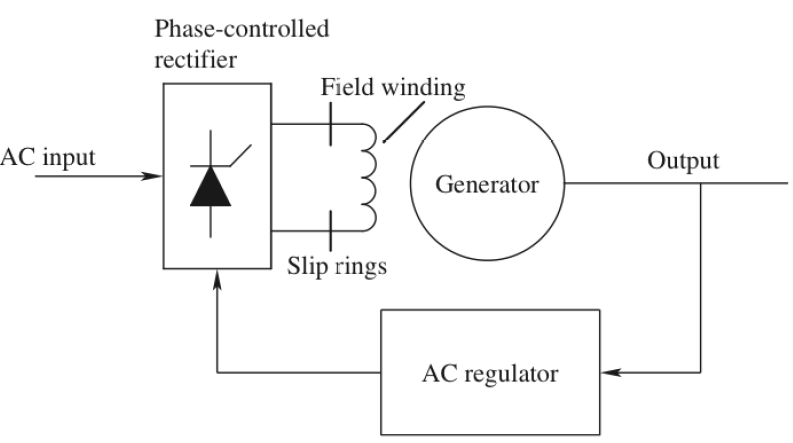
\includegraphics[width=\textwidth]{exciter.png}
        \end{column}
        \begin{column}{0.6\textwidth}
            \includegraphics[width=\textwidth]{avr.png}
        \end{column}
    \end{columns}
    \tiny{Figure on the right from: Voltage stability of electric power systems. T. Van Cutsem \& C. Vournas, KAP 1998}
    \begin{itemize}
        \item Notice that if several generators are connected in parallel (either at the MV or at the EHV bus), it is necessary to coordinate their AVRs so that they share the reactive power in an even way.
        \item The value of $Z_c$ may be adjusted in order to ensure such a coordination.
    \end{itemize}
\end{frame}

% Primary, secondary and tertiary voltage control
\begin{frame}
    \frametitle{Primary, secondary and tertiary voltage control}
    \begin{itemize}
        \item When a disturbance occurs, or subsequently to following the change in load (cf. 'duck curve'), the \textit{primary} voltage control loops maintain suitable voltage levels close to the large power plants equipped with AVRs.
        \begin{itemize}
            \item However, voltages at other buses may move out of tolerance intervals (in either direction), and reactive power reserves may not be shared in an even way among generators.
        \end{itemize}
        \item \textit{Secondary} voltage control loops can be used at the zonal level, to adjust the set-points of AVRs so as to control the voltage at 'pilot nodes' in the network while distributing the required reactive power evenly among generators.
        \begin{itemize}
            \item Secondary voltage control loops can also be used to switch shunt reactive compensation devices (capacitors/inductors) in order to increase reactive power generation margins in their zone (among a few large power plants).
        \end{itemize}
        \item \textit{Tertiary} voltage control uses OPF solvers to calculate set-points at pilot nodes and possibly adjust some transformer ratios, so as to minimize losses and maximize MVar reserves at the entire system level.
        \item Response times of different levels of voltage control
        \begin{itemize}
            \item \textit{Primary:} 1-3 seconds ; \textit{Secondary:} 30 seconds -3 minutes ; \textit{Tertiary:} 10-15 minutes
        \end{itemize}
    \end{itemize}
\end{frame}

\begin{frame}{Control resources}

    Which of these control resources are the main levers for freqency stability?
      \begin{itemize}
          \item Adjust synchronous generators' field current
          \item \alert{Adjust synchronous generators' mechanical power}
          \item Change transformer taps
          \item Change shunt compensation
          \item Act on topology: switch lines and transformers in/out of service
          \item \alert{Fast start-up generator units}
          \item \alert{In extremis load curtailment}
          \item \alert{Control renewable generation (e.g. PV curtailment)}
          \item \alert{Use batteries and other energy storage systems} %TODO Ask ELIA to which reserve markets batteries are participating
      \end{itemize}
\end{frame}